\chapter{Performance test}\label{S:Performance-Test}
In this chapter the results for a GPIO performance tests are shown. This tests will be done using the Raspberry Pi and two implementations of IOSharp, the original written in C\# which has been explained on the first part of this thesis, the second implementation tested will be the C++ one translated from the original by AlterNative which has been explained in the second part of this thesis. Theoretically, C++ has a major performance compared to C\# but this tests are used to determine how much the C++ implementation gains over the C\# ones.
\\
To make the measures in this tests the Logic16 has been used. This is a channel analyzer used to record, view, and measure digital signals. It also currently has 17 different protocol analyzers including SPI, serial, I2C and many more.

\section{GPIO}\label{SS:IOEx-GPIO}
The GPIO test consists on how much time takes the board to perform a certain number of iterations changing an output port between the high and low states. Two channels are used in this test, the first one will activate the Logic to start sniffing the second channel which will be the one that performs the output between the two states.
\\
The code used in this test is shown below, both the original version and the translated one using AlterNative.
\begin{lstlisting}[language=CSharp, caption={GPIO Performance test in C\#}]
using System;
using System.Collections.Generic;
using System.Linq;
using System.Text;
using Microsoft.SPOT.Hardware;
using IOSharp.NETMF.RaspberryPi.Hardware;
using System.Threading;

namespace raspberrypi
{
    class Program
    {
        public static void Main()
        {
            Debug.Print("START");
            OutputPort bar = new OutputPort(Pins.V2_GPIO17, false);
            bar.Write(false);
            bool foo = false;
            OutputPort o = new OutputPort(Pins.V2_GPIO11, false);

            bar.Write(true);
            for (int i = 0; i < 10000; i++)
            {
                foo = !foo;
                o.Write(foo);
            }
            bar.Write(false);
            Debug.Print("END");
        }
    }
}
\end{lstlisting}

\begin{lstlisting}[language=C++, caption={GPIO Performance translated to C++}]
#include "Program.h"
namespace raspberrypi {

	void Program::Main(){
		Program* p = new Program();
		p->Run();
	}

	void Program::Run(){
		Debug::Print(new String("START"));
		OutputPort* bar = new OutputPort(Cpu::Pin::GPIO_Pin17, false);
	
		bar->Write(false);
		bool foo = false;
		OutputPort* o = new OutputPort(Cpu::Pin::GPIO_Pin11, false);
		bar->Write(true);
		for (int i = 0; i < 200; i += 1) {
			Debug::Print(new String(i));
			foo = !foo;
			o->Write(foo);
		}
		bar->Write(false);
		Debug::Print(new String("END"));
	}
}
\end{lstlisting}

This test will be executed varying the number of iterations between 200 and 10000. Each iteration will swap the port between high and low. Apart from the iteration increase, two type of compilations will be done changing the optimization type between quick compilation without optimization (Debug) and compilation with optimization (Release).

\subsection{200 Iterations}\label{SS:200-iterations}
The result produced by Mono shows an irregular pattern consisting of two small pulses a wide pulse and then two small pulses following a wide gap. This pattern is regularly repeated across all the test. The wide pulses and gaps are supposed to be caused by the garbage collector and the thread hopping of mono.
\\
The small pulses are around \textcolor{red}{5ms} and the wide gaps/pulses are \textcolor{red}{10ms}. Each block is repeated every \textcolor{red}{20ms}.

\begin{figure}[H]\begin{center}
 \centering
  \captionsetup{justification=centering}
  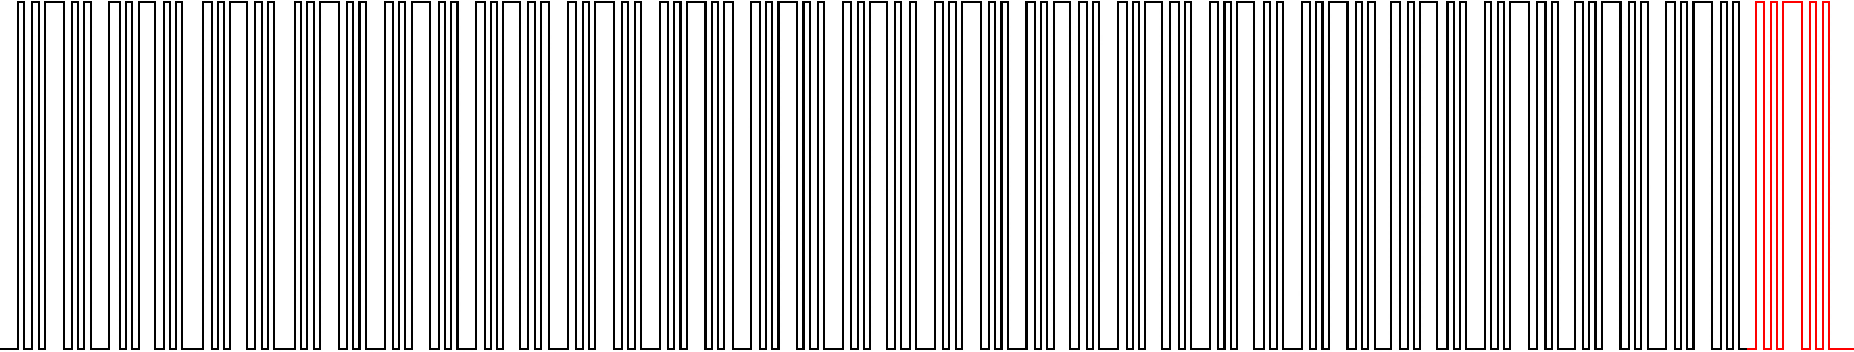
\includegraphics[width=1\textwidth]{pictures/performance-tests/GPIO/200/csharp}
  \caption{200 Iterations using C\# with optimizations \label{fig:gpio-200it-csharp}}
\end{center}\end{figure}

In case of the C++ test it can be observed that the pulses are much more regular than the mono test, but at certain point around the pulse 89 a big gap is observed probably due to the lack of a garbage collector in the programs generated by AlterNative.

\begin{figure}[H]\begin{center}
 \centering
  \captionsetup{justification=centering}
  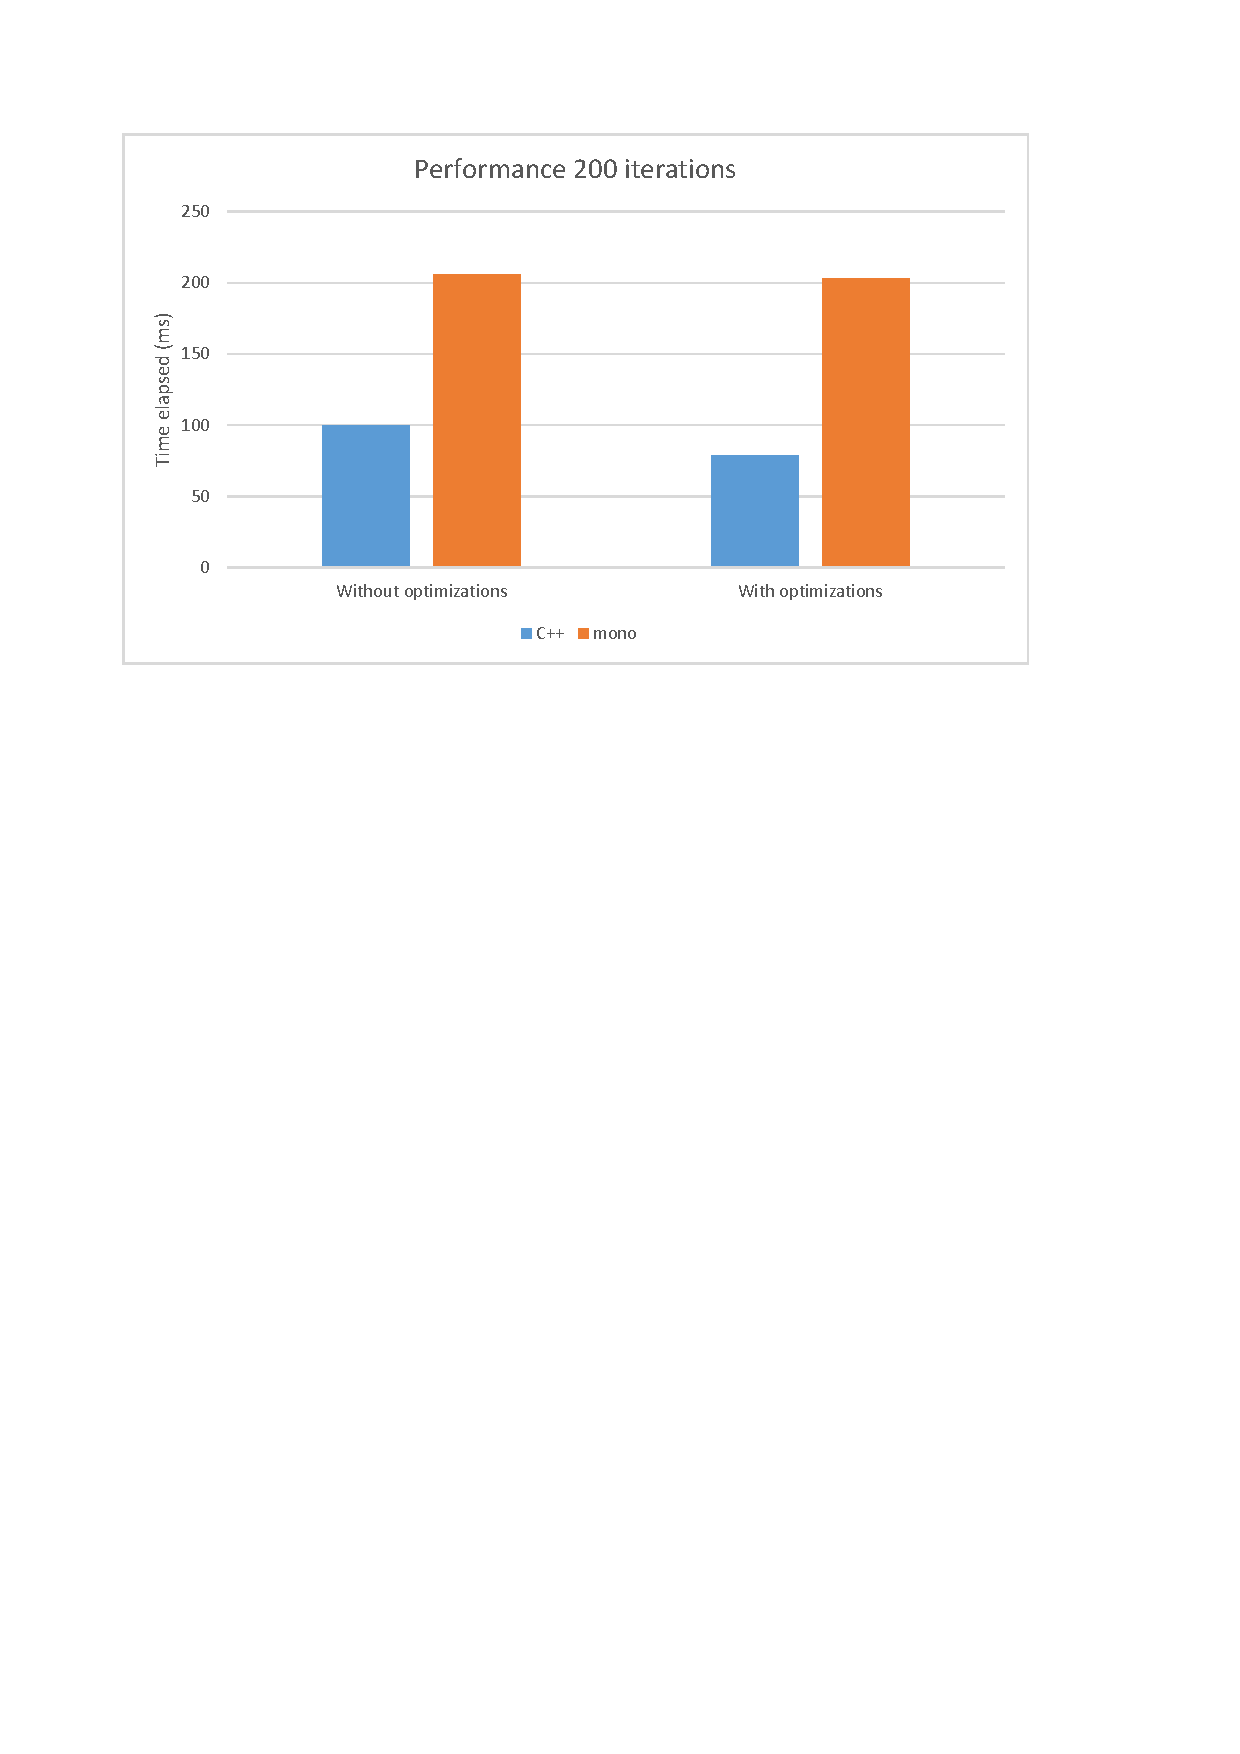
\includegraphics[scale=0.9,page=1]{pictures/performance-tests/GPIO/graphs}
  \caption{Graph showing the elapsed time for the 200 iteration test. Blue is for C++ while orange is C\#. On the left is represented the non-optimized compilations and on the right the optimized ones\label{fig:gpio-graph-200}}
\end{center}\end{figure}

\subsection{10K Iterations}\label{SS:10K-iterations}

\begin{figure}[H]\begin{center}
 \centering
  \captionsetup{justification=centering}
  \includegraphics[scale=0.9,page=2]{pictures/performance-tests/GPIO/graphs}
  \caption{Graph showing the elapsed time for the 10k iteration test. Blue is for C++ while orange is C\#. On the left is represented the non-optimized compilations and on the right the optimized ones\label{fig:gpio-graph-10k}}
\end{center}\end{figure}

\section{Interruptions}\label{SS:IOEx-Interruptions}
\textcolor{red}{we expect this to work}